\section{Theory}
\label{sec:theorem}
In this section, we elaborate the origin, the intuition, and the experimental basis behind Eq.~\ref{eq:scaling}. We then validate our formula through extensive experiments.

\subsection{Similarity between Learning Rate, Gradient Norm, and Loss}

\begin{figure}[tbp]
\centering
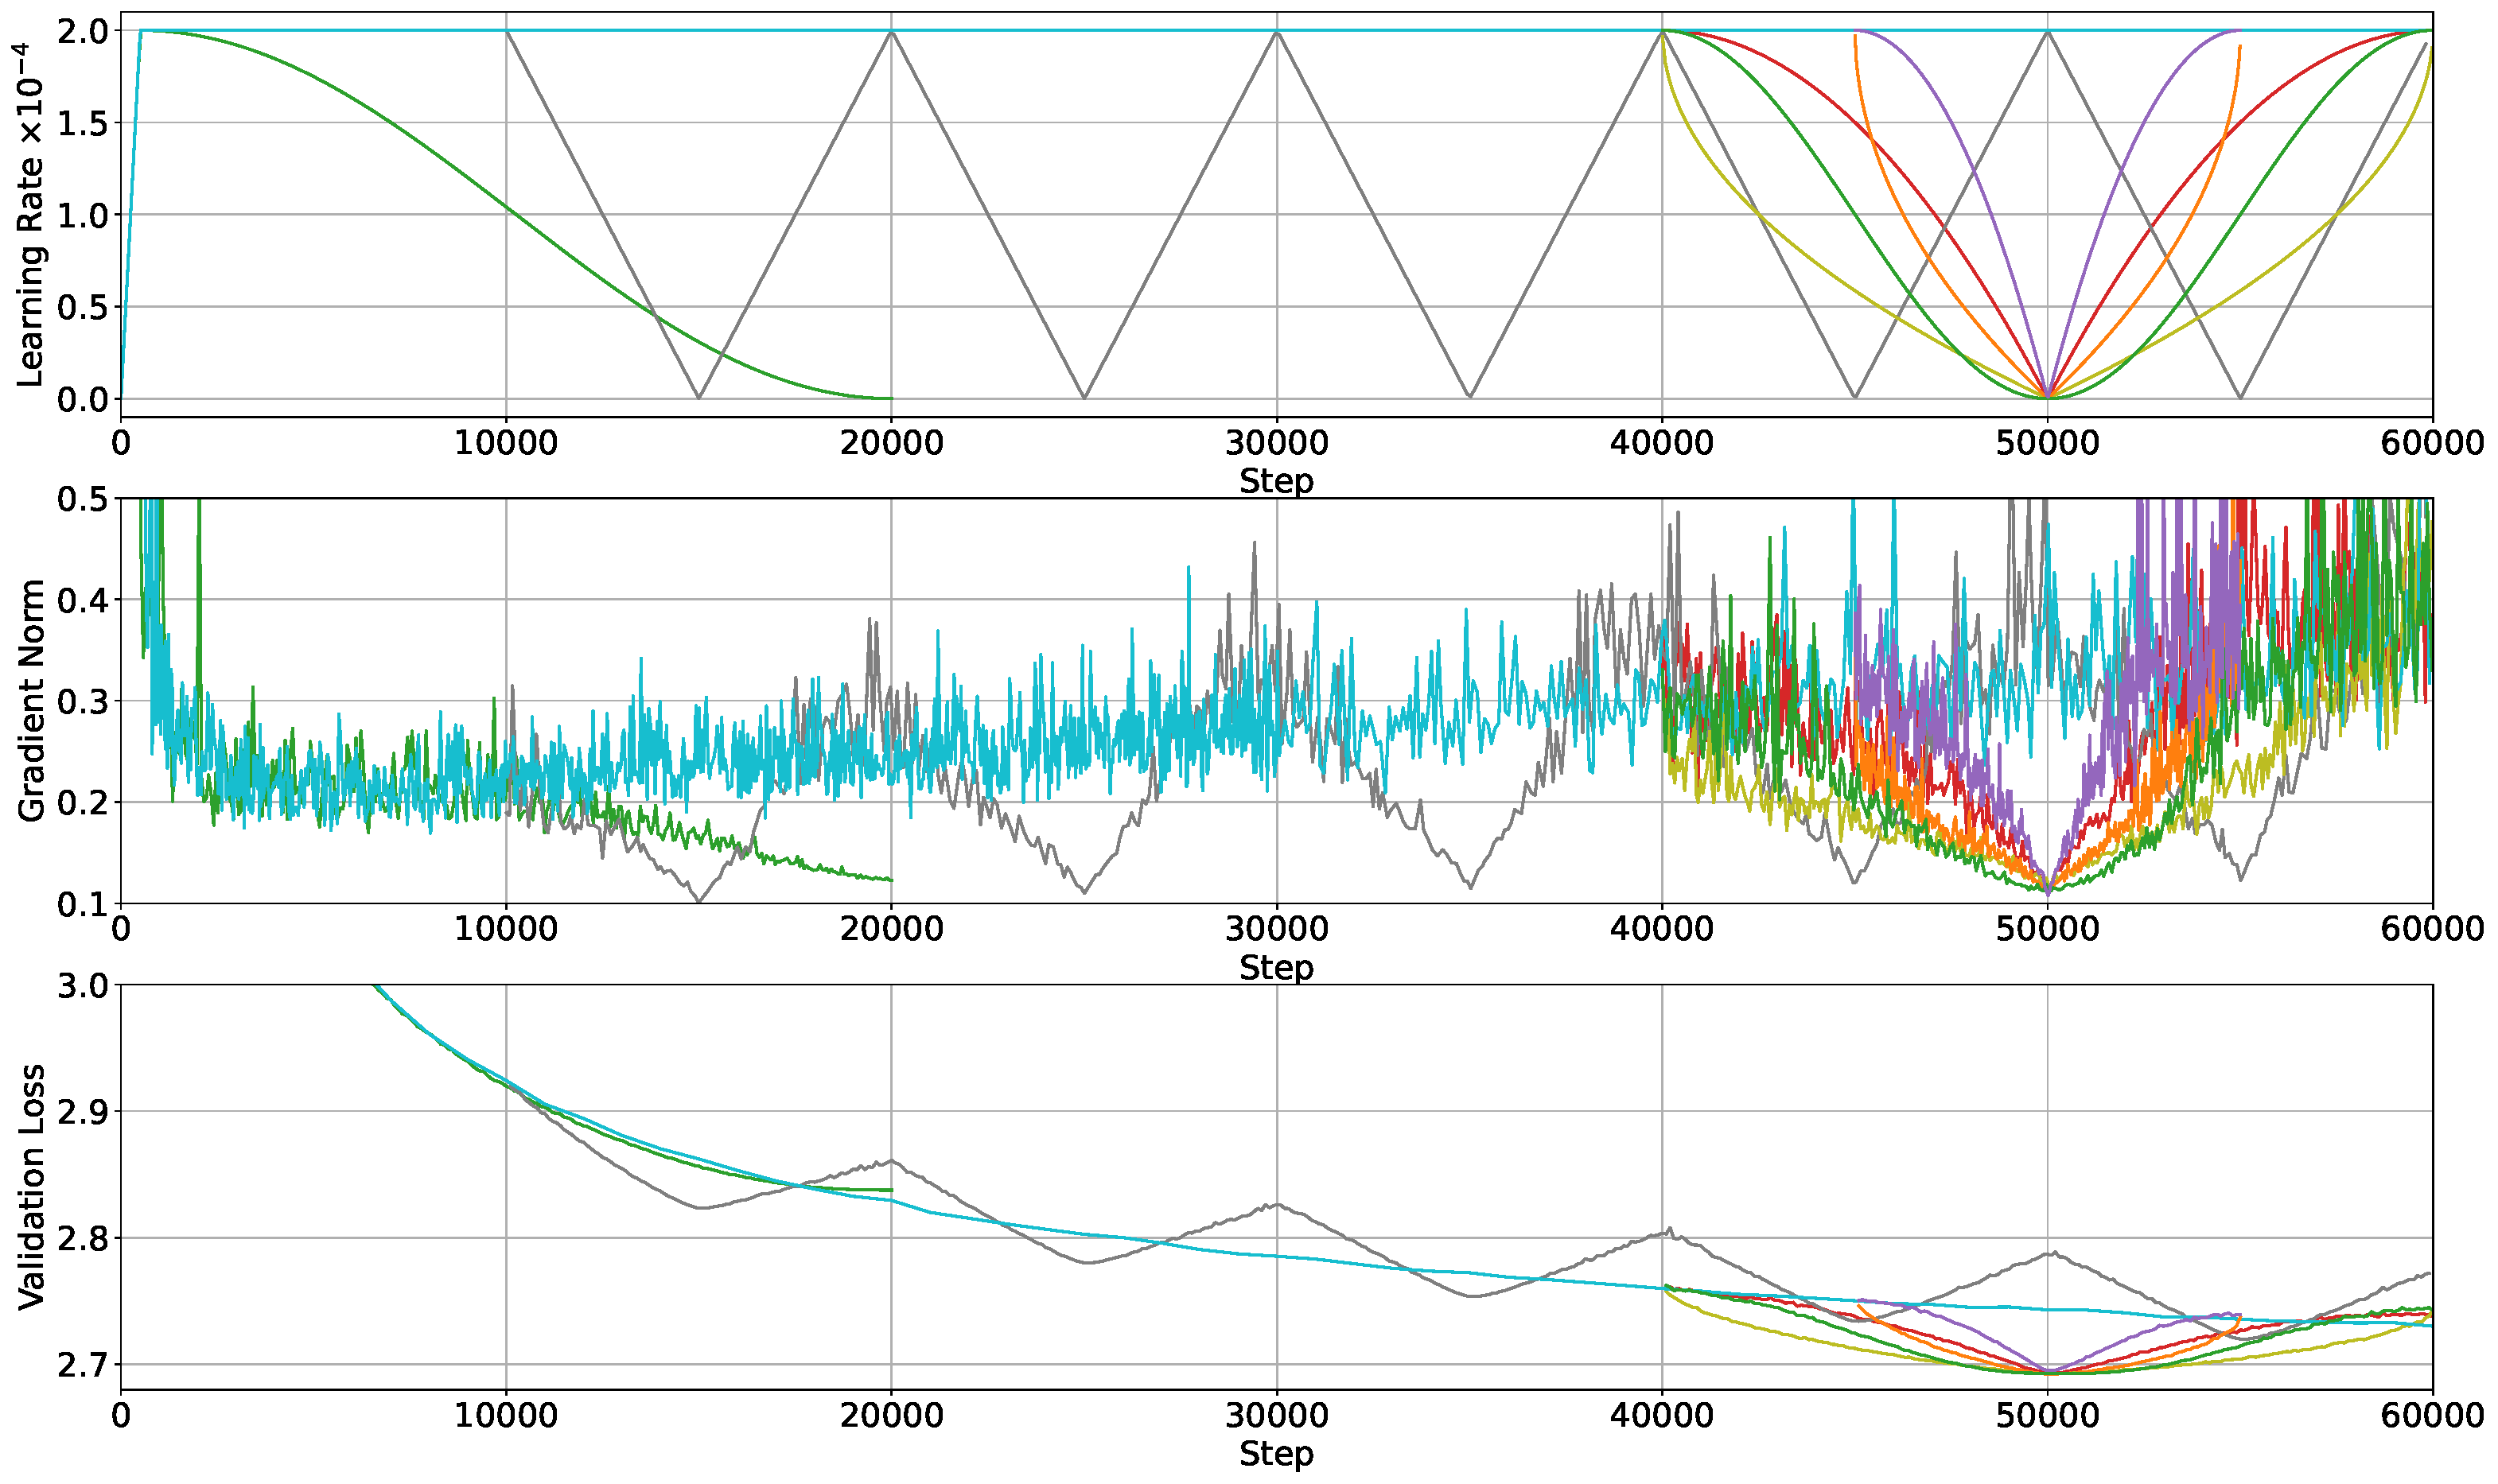
\includegraphics[width=0.95\linewidth]{images/draw_phe/7.pdf}
\caption{The shapes of LR (top), gradient norm (medium), and validation loss (bottom) curves exhibit high similarity across various LRS (labeled as different colors).}
\label{fig:similarity}
\end{figure}

The first key observation is that the shapes of LR curve, gradient norm curve, and validation loss curve are quite similar across various LRS when training LLMs (Fig.~\ref{fig:similarity}). This suggests an implicit connection between learning rate and loss, where gradient norm could be the bridge.

\paragraph{Scaling Laws for Constant LRS.}
A constant LRS is a special LRS, where every training step can be viewed as an endpoint of the LRS. Notably, the Chinchilla scaling law~\citep{hoffmann2022training} exactly fits losses of last steps, i.e., LRS endpoints. 
Therefore, the expectation of validation loss of all steps under in constant LRS adheres to a power-law over training step $s$.

\paragraph{Extra Loss Changes in LR Annealing.}
Unlike a constant LRS, LR annealing (or re-warmup) brings significant local changes in the loss (see Fig.~\ref{fig:similarity}), causing the full loss curve to deviate from the traditional power-law formulation that consider only the training steps $s$. We hypothesis that such loss changes can be captured by an additional LR ($\eta$) related term, i.e.,
\begin{equation}
\begin{aligned}
L(s) = {\color{cyan} \underbrace{L_0 + A\cdot s^{-\alpha}}_{\text{Traditional scaling law}}} 
\quad
{\color{red} \underbrace{-f(\eta)}_{\text{LR annealing term}}},
\end{aligned}
\label{eq:guess-1}
\end{equation}
where the first two terms (blue part) follow traditional scaling laws, while the last term (red part) denotes the extra loss change brought by LR annealing. Recall the similarity between learning rate and loss curves, we can form a naive guess for $f(\eta)$ as $f(\eta) = C\cdot\eta_s$, where $C$ is a positive constant.

\paragraph{Training Discount in Annealing.} The form of Eq.~\ref{eq:guess-1} is still imperfect. 
Note that the gradient norm $\Vert \mathbf{g} \Vert$ decreases along with LR during the annealing process (shown in Fig.~\ref{fig:similarity}).
Thus, the amount of parameter movement (approximately $\eta \cdot \Vert \mathbf{g} \Vert$ per step) in the LR annealing stage declines at an almost quadratic rate compared to stages before annealing.
As the parameter movement become smaller, the change in loss also slows down accordingly. Therefore, the loss drop brought by the power law term (i.e., the first two terms in Eq.~\ref{eq:guess-1}) should also diminish during LR annealing. 
This consideration leads to an improved equation:
\begin{equation}
\begin{aligned}
L(s) &= {\color{cyan} L_0 + A\cdot S_1^{-\alpha}} {\color{red} - f(\eta)} \\
S_1 &=  \sum\limits_{i=1}^{s}\eta_i,
\end{aligned}
\label{eq:guess-2}
\end{equation}
where $S_1$ is the forward area, i.e., the area under the LR curve (as visualized in Fig.~\ref{fig:definition}), which could be approximately interpreted as the total amount of parameter updates.

\subsection{LR Annealing Momentum}
\begin{figure}[tbp]
    \centering
    \begin{subfigure}[b]{0.48\textwidth}
        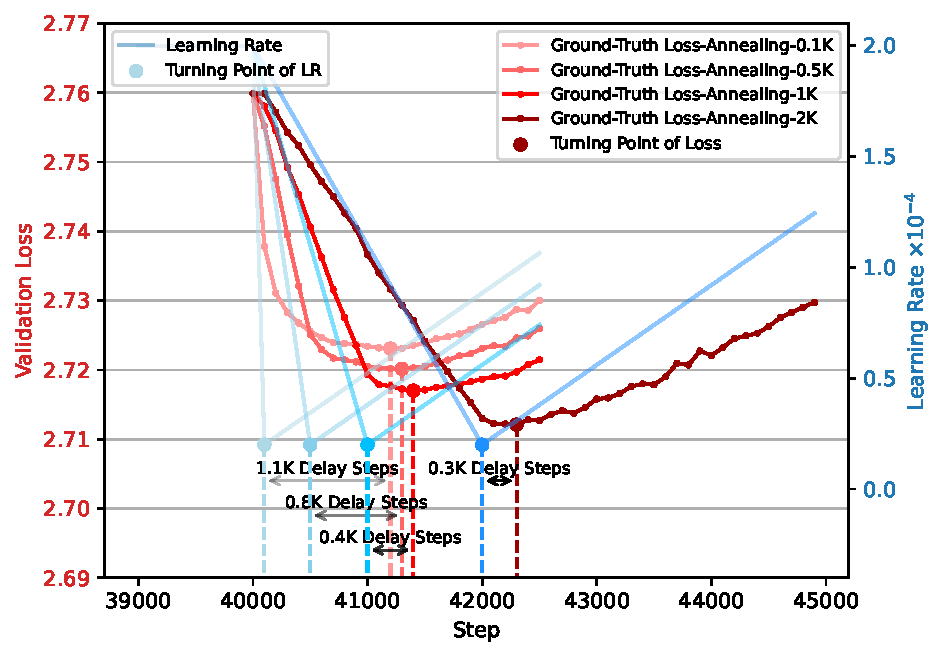
\includegraphics[width=\textwidth]{images/plot_newxy/decrease.pdf}
        \caption{Different delay steps in the annealing process associated with different annealing steps (0.1K, 0.5K, 1K and 2K).}
        \label{fig:delay-anneal-then-rewarmup}
    \end{subfigure}
    \hfill
    \begin{subfigure}[b]{0.48\textwidth}
        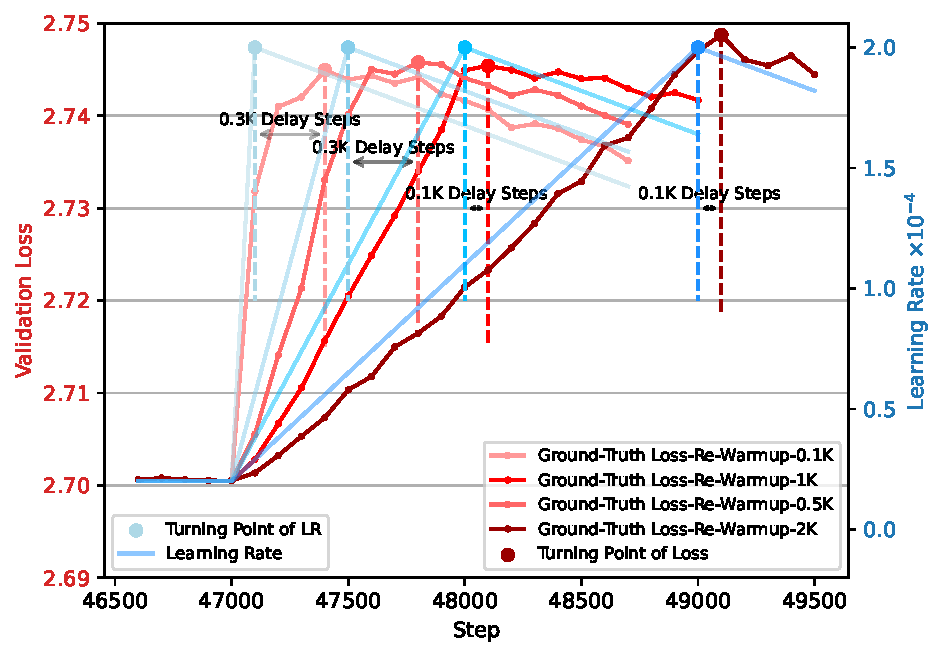
\includegraphics[width=\textwidth]{images/plot_newxy/increase.pdf}
        \caption{Different delay steps in the re-warmup process associated with different re-warmup steps (0.1K, 0.5K, 1K and 2K).}
        \label{fig:delay-rewarmup-then-anneal}
    \end{subfigure}
    \caption{The delay phenomenon between the LR and validation loss curves. This phenomenon suggests that LR annealing (re-warmup) has momentum.}
\label{fig:delay}
\end{figure}

Another key observation is that LR annealing has momentum.
To refine the formulation of $f(\eta)$,
we design a special LRS where the LR decreases linearly from $\eta_{max}$ to $\eta_{min}$ and then increases.
The increasing stage always has a fixed slope, reaching the maximum value in 5K steps, while the slope of the decreasing stage is varied, with durations of 0.1K, 0.5K, 1K, and 2K. 
Symmetrically, we design another LRS where the LR increases linearly from $\eta_{min}$ to $\eta_{max}$ and then decreases. Fig.~\ref{fig:delay} shows the corresponding LR and loss curves.

We observe a \textbf{delay phenomenon} between the LR and the validation loss. Firstly, the turning point of the validation loss curve consistently lags behind the turning point of the LR curve, indicating that the validation loss continuous along its previous trajectory for some steps even after the LR changes direction. Secondly, the steeper the slope of the LR annealing (or re-warmup), the more pronounced the delay phenomenon becomes. 
Thirdly, given the same LR slope, the left figure (where LR decreases then increases) consistently shows a longer delay compared to the right figure (where LR increases then decreases). We discuss some possible root reasons of delay phenomenon in Sec.~\ref{sec:discsussion-delay}.

Interestingly, this phenomenon closely resembles the physical experiment of a small ball rolling down a slope.
The steeper the slope, the faster the ball accelerates. 
When the ball lands, the accumulated momentum causes the ball to slide further.
Inspired by this delay phenomenon, we hypothesize that $f(\eta)$, the loss reduction induced by LR annealing, has cumulative historical formation so that the past change of learning rate will affect the following
loss curve for a few steps.
In summary, \emph{learning rate annealing exhibits momentum}. 
To capture this, we define $f(\eta) = C\cdot S_2$, where $S_2$ is calculated as:
\begin{equation}
\label{eq:definition-s2}
\begin{aligned}
    m_i &= \lambda \cdot m_{i-1} + (\eta_{i-1} - \eta_i), \\
    S_2 &= \sum\limits_{i=1}^{s}m_i = \sum\limits_{i=1}^{s}\sum\limits_{k=1}^{i}(\eta_{k-1} - \eta_{k})\cdot \lambda^{i-k},
\end{aligned}
\end{equation}
where $m_i$ is the LR annealing momentum at step $i$ ($m_1=0$), and $\Delta \eta = \eta_{i-1} - \eta_i$ denotes the LR annealing amount at step $i$. $\lambda$ is the decay factor that signifies how much historical information is retained. 
We find that $\lambda$ values between $0.99$ and $0.999$ generally works well. 
In contrast, $\lambda=0$ implies no momentum effect, reducing $f(\eta)$ to $C\cdot\eta_s$, which degenerate to the initial form mentioned above. 
Note that $S_2$ applies not only to LR annealing ($S_2>0$), but also to LR re-warmup ($S_2<0$). This means that our equation is applicable to scenarios like continual pre-training, where LR re-warmup serves
as an important factor for better outcomes (see Sec.~\ref{sec:takeaways}). 
More intuitively, the definition of $S_2$ can be visualized
in Fig.~\ref{fig:definition}, as the weighted sum of blue grid areas.


\subsection{Final Formulation}
\paragraph{Scaling Law with LR Annealing.}
\emph{Given the same training and validation dataset, the same model size, the same training hyper-parameters such as warmup steps, max learning rate $\eta_{max}$ and batch size, the language modeling loss at training step $s$ empirically follows the equation $L(s) = L_0 + A\cdot S_1^{-\alpha} - C\cdot S_2$, where $S_1$ and $S_2$ are defined in Eq.~\ref{eq:scaling}. $L_0$, $A$, $C$, $\alpha$ are positive constants.}

Our formulation describes the loss of each training step across different LRS. It allows fitting based on a simpler LRS with shorter training steps and enables the prediction of validation losses for more complex LRS with longer training steps.


\begin{wrapfigure}{r}{0.45\linewidth}
    \centering
    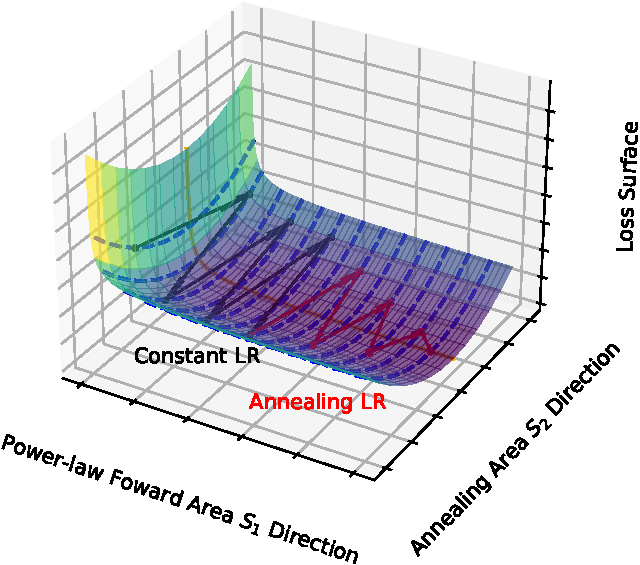
\includegraphics[width=\linewidth]{images/slide-crop.pdf}
    \caption{Loss surface of language models as a \emph{slide} after simplification. Optimization direction could be decomposed into two directions: power-law scaling direction ($S_1$, sliding down) and annealing direction ($S_2$, inner height of the slide).}
\label{fig:slide}
\end{wrapfigure}

\paragraph{Only {\color{red} One Extra} Parameter.} Notably, we add only one parameter, the coefficient of $S_2$ term $C$, compared to Chinchilla scaling law~\citep{hoffmann2022training}. 
%Theoretically, enough parameters can always fit any curve but cannot generalize to unseen curve prediction. 
That is, we utilize the fewest extra parameters but model the essential training dynamics in LR annealing to the greatest extent.

\paragraph{Loss Surface as a Slide.} To better understand our formulation, we view the loss surface of language models as a slide in Fig.~\ref{fig:slide}. The optimization process can be seen as sliding down the slide according to the power-law scaling ({\color{orange} orange line}), while oscillating on the inner wall ({\color{blue} blue dashed line}). When the learning rate anneals ({\color{red} red line}), the amplitude of the oscillation decreases, resulting in a reduction in loss.


% \begin{figure}[tbp]
%     \centering
%     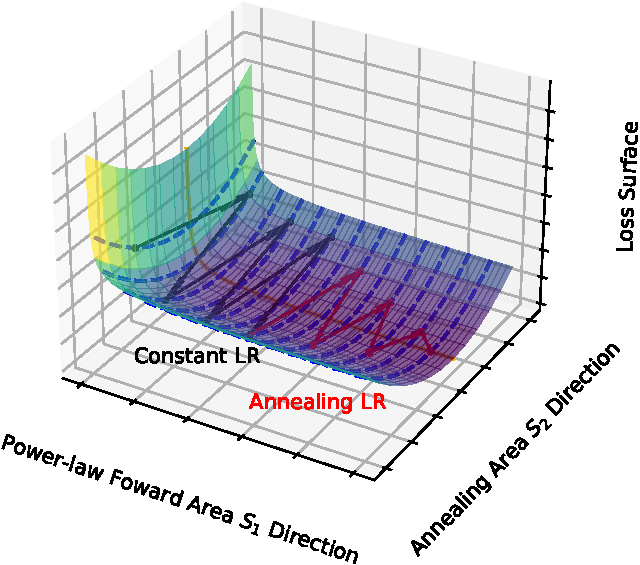
\includegraphics[width=0.8\linewidth]{images/slide-crop.pdf}
%     \caption{Loss surface of language models as a \emph{slide} after simplification. Optimization direction could be decomposed into two directions: power-law scaling direction ($S_1$, sliding down) and annealing direction ($S_2$, inner height of the slide).}
% \label{fig:slide}
% \end{figure}

\paragraph{Balance between $S_1$ and $S_2$.}
Note that in Eq.~\ref{eq:scaling}, $\frac{\partial L}{\partial S_1}<0$ and $\frac{\partial L}{\partial S_2}<0$ always hold, indicating that increases in both $S_1$ and $S_2$ help to reduce the loss.
However, as shown intuitively in Fig.~\ref{fig:definition}, there exists delicate balance between $S_1$ and $S_2$. When LR begins to anneal and $S_2$ starts to increase, the forward area $S_1$ of subsequent steps starts to diminish instead. 
Our equation aptly describes this delicate balance.
In Sec.~\ref{sec:takeaways}, we elaborate this topic in detail.
\subsection{Experiments}
\paragraph{LR Warmup.} Different warmup steps can result in different loss curves in training from scratch.
During the warmup stage, neural networks are prone to random optimization, resulting in \emph{unpredictable} outcomes~\citep{hestness2017deep}.
Various studies, along with our own pilot experiments (Appendix~\ref{apx:warmup}), show that LR warmup significantly accelerates model convergence.
High gradient norms are usually observed during the LR warmup stage, especially in the initial steps of training (see Fig.~\ref{fig:similarity}). This indicates that model parameters undergo substantial updates during this stage.
% shows that the gradient norm decreases sharply in the first few training steps.  
% is necessary for convergence. Our pilot experiment (refer to Appendix~\ref{apx:warmup}) shows that warmup indeed significantly accelerates convergence. 
%, a finding also noted by~\citet{warmup-evidence,kosson2024analyzing}. 
Therefore, in all our experiments, we linearly warmup LR to reach $\eta_{max}$ but compute $S_1$ and $S_2$ assuming a constant LR value $\eta_{max}$ in the warmup stage.

\paragraph{Experimental Setups.}
We use standard experimental setups for LLM pre-training. In our main experiments,
the training dataset is Fineweb~\citep{penedo2024fineweb} and the validation
dataset is RedPajama-CC~\citep{together2023redpajama}. We train a $594$M non-embedding parameters LLAMA
architecture-like model~\citep{touvron2023llama} from scratch. We use AdamW optimizer~\citep{loshchilov2017decoupled} with $\beta_1 = 0.9$ and $\beta_2 = 0.95$. The weight decay is set as $0.1$ and gradient clip is set as $1.0$. We set maximal learning rate as $2\times10^{-4}$ and batch size as $4$M tokens.
To verify the robustness of our formulation across different experimental settings, we have four other distinct experimental setups (see Appendix~\ref{apx:exp-sets}). 
We adopt the decay factor or learning rate annealing $\lambda=0.999$ in our all experiments and discuss the impact of $\lambda$ in Sec.~\ref{sec:discsussion-lambda}.

\paragraph{Fitting Details.}
Given a LRS of total step $s$, i.e., a learning rate value sequence $\{\eta_1, \eta_2\, \cdots, \eta_s\}$, the value of $S_1$ and $S_2$ for each step can be computed using Eq.~\ref{eq:scaling} in advance.
To estimate $(L_0, A, C, \alpha)$, we adopt a similar fitting method as used by~\citet{hoffmann2022training}. Specifically, we minimize the Huber loss~\citep{huber-loss} between the predicted and the observed log loss values using the L-BFGS algorithm~\citep{L-BFGS}:
\begin{equation}
\label{eq:huber}
\begin{aligned}
\min_{L_0,A,C,\alpha}\quad\sum_{\mathrm{Step~} i}\mathrm{Huber}_\delta\left(\log\hat{L}(i)-\log L(i)\right).
\end{aligned}
\end{equation}
We use the implementation of the \texttt{minimize} method provided by the \texttt{scipy} library. Huber loss is to enhance the robustness of the fitting process and we set the $\delta$ value of Huber loss to $1.0\times 10^{-3}$. To address the potential issue of local minima during fitting, we select the optimal fit by testing across a range of initial conditions. Note that in practice, we can also fit the loss curves generated by multiple LRS using the same set of parameters $(L_0, A, C, \alpha)$. In this situation, we sum the Huber losses from Eq.~\ref{eq:huber} of all fitted LRS.

\paragraph{Fitting and Prediction Results.}
We fit Eq.~\ref{eq:scaling} on the loss curves under constant and cosine LRS with 20K total steps (see Fig.~\ref{fig:fit}), and then predict the full loss curves under several unseen LRS with 60K total steps (see Fig.~\ref{fig:prediction}). The results show an almost perfect fit, achieving a coefficient of determination ($R^2$) greater than $0.999$. This underscores the robust capability of our equation to accurately fit loss curves across diverse LRS using a single parameter tuple.

The prediction results in Fig.~\ref{fig:prediction} indicate that our formulation is broadly applicable and  generalizes robustly across four unseen LRS, with a mean prediction error as low as 0.2\%. Moreover, our equation can accurately predict losses even for complex LRS that include multiple LR re-warmup stages (Fig.~\ref{fig:prediction-strange}), despite that the loss curves used for fitting do not contain any LR re-warmup stages.

\paragraph{Extensive Experiments on Different Setups.}
To demonstrate the broad applicability of our proposed equation, we conduct additional fitting and prediction experiments using various setups. (1) We use an alternative set of training hyper-parameters (Appendix~\ref{apx:exp-2}); (2) We test our equation on the Mixture of Experts (MoE) architecture (Appendix~\ref{apx:moe}); (3) We apply our equation to predict loss curves for a much longer ($10\times$) training run involving a 1.7B parameter model trained on 1.4T tokens (Appendix~\ref{apx:long-exp}).
(4) We fit the loss curves of open-sourced models, including BLOOM-176B trained on 300B tokens \citep{workshop2022bloom} and OLMo-1B trained on 2T tokens ~\citep{groeneveld2024olmo} (Appendix~\ref{apx:open-source}).
All experiments produce excellent results, indicating that our equation is effective across diverse experimental setups, including different training hyper-parameters, architecture, model sizes, and dataset scales.

\begin{figure}[tbp]
    \centering
    \begin{subfigure}[b]{0.48\textwidth}
        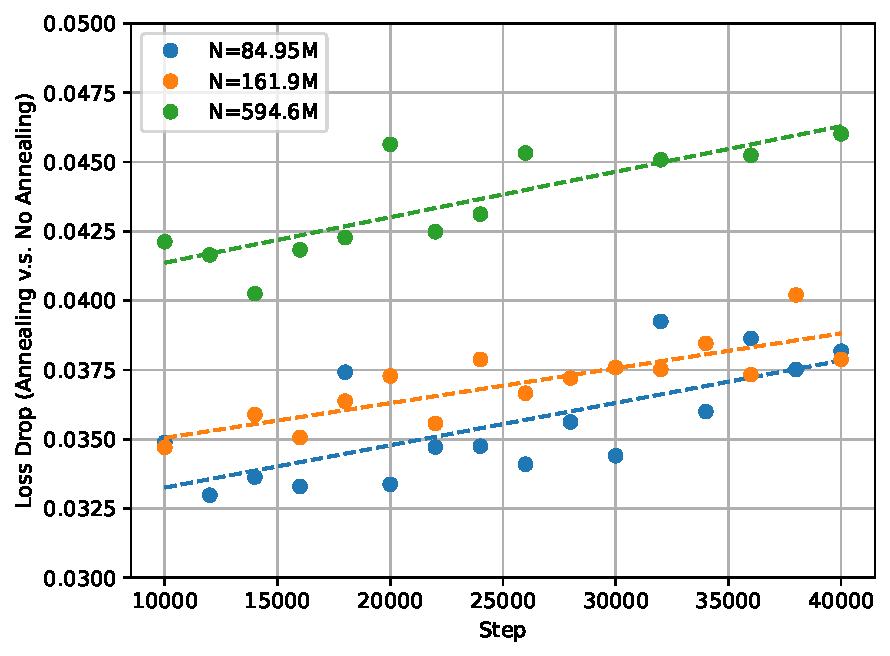
\includegraphics[width=\textwidth]{images/draw_phe/5.pdf}
        \caption{The loss drop brought by LR annealing for different model size $N$. Dashed lines represent trends over steps. The loss drop brought by LR annealing scales with data size and model size.}
        \label{fig:delta-N}
    \end{subfigure}
    \hfill
    \begin{subfigure}[b]{0.48\textwidth}
        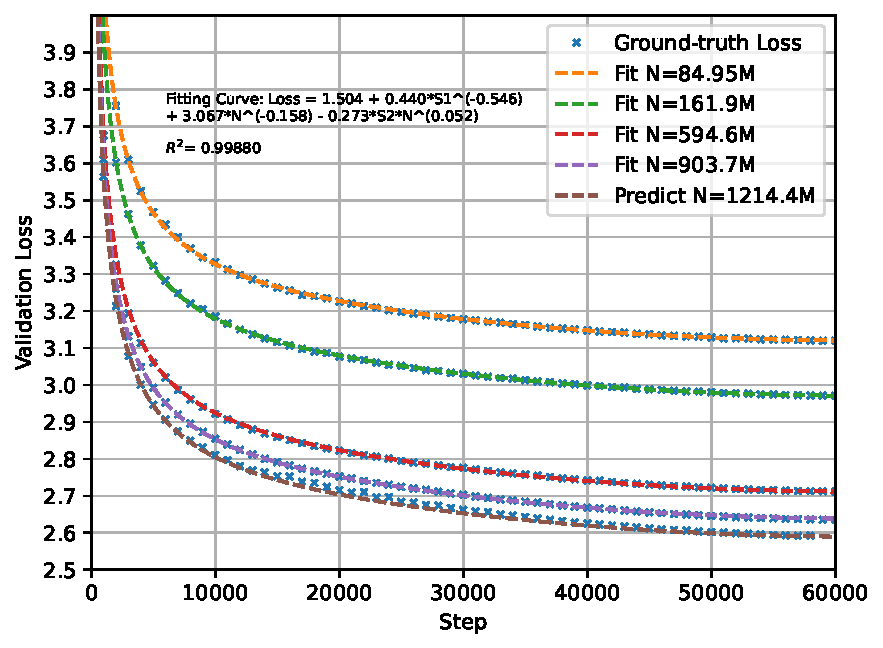
\includegraphics[width=\textwidth]{images/draw_phe/6-predict.pdf}
        \caption{Curve fitting and prediction on cosine LRS (60K steps to $\eta_{min}=0.1\cdot\eta_{max}$) of different model sizes using our $N$-extended scaling law. Results for N=1214.4M are predicted.}
        %Substituting specific values of $N$ can simplify to Eq.~\ref{eq:scaling}.}
        \label{fig:scaling-N-fit}
    \end{subfigure}
    \caption{The loss drop brought by LR annealing (left) and the $N$-extended full loss curve fitting and prediction (right). It suggests that $S_2 \propto N^\gamma$ is reasonable from both experimental phenomena and accurate curve prediction.}
\end{figure}

\subsection{Extension to Model Size Scaling}
\paragraph{Loss Drop During Annealing Scales with Model Size $N$.}
We explore the effect of model size $N$ on the loss drop during the annealing stage. Specifically, we compare the final losses obtained with a constant LRS and a WSD LRS (10\% cosine annealing to $\eta_{min}=0$) to estimate the loss drop due to LR annealing. We conduct this experiment on different total steps and different model sizes. The experimental results are shown in Fig.~\ref{fig:delta-N}. It suggests that the loss drop from LR annealing scales with both annealing steps and model sizes. This implies that the annealing area $S_2$ in our equation should also increase as the model size $N$ increases. We suppose there is a simple relationship of $S_2 \propto N^\gamma$ where $\gamma$ is a positive constant.


\paragraph{Model Size Scaling.} Building on the experiments and analysis above, we extend our proposed Eq.~\ref{eq:scaling} to incorporate model size scaling, based on traditional scaling laws (Eq.~\ref{eq:chinchilla}):
\begin{equation}
\begin{aligned}
& L(s, N) = L_0 + A\cdot S_1^{-\alpha} + B\cdot N^{-\beta}- C\cdot S_2 \cdot N^{\gamma},
\end{aligned}
\label{eq:scaling-N}
\end{equation}
where $N$ is the number of non-embedding model parameters, and $B$, $\beta$, $\gamma$ are positive constants related to $N$.
We parameterize $S_2 \propto N^{\gamma}$ via a multiplier $N^{\gamma}$ to the original annealing term $-C\cdot S_2$.

\paragraph{Fitting and Prediction with Model Size.}
We validate Eq.~\ref{eq:scaling-N} by fitting the full loss curves of models with varying sizes.
We then apply the obtained equation to predict full loss curve on the unseen largest model size.
Results in Fig.~\ref{fig:scaling-N-fit} show an almost perfect fit ($R^2>0.998$) and prediction for entire training dynamics of larger-scale models. This indicates the effectiveness and robustness of our proposed $N$-extended equation.
Additional $N$-extended experiments with other setups further confirm the robustness of our formulation (see detail in Appendix~\ref{apx:exp-2-N}).